\documentclass[12pt]{article}
\usepackage{fullpage}
\usepackage{lineno}
\usepackage[notcite,notref]{showkeys}
\usepackage[notcite,notref]{showkeys}
\usepackage{amssymb}
\usepackage{amsmath}
\usepackage{natbib}

\usepackage{epsfig}
\usepackage[mathscr]{eucal}



\bibliographystyle{plain}

%% For lucida bright
%\usepackage[T1]{fontenc}
%\usepackage{lucidabr}
%\usepackage{bm}
%%%




\usepackage{color,amssymb,amsmath,amsthm}

\usepackage{epsfig}
\usepackage[mathscr]{eucal}


\newcommand{\NIW}{near-inertial wave}
\newcommand{\macrot}{macroturbulence}

\newcommand{\com}{\, ,}
\newcommand{\per}{\, .}

%% Averages
% Use \bar to over line solo symbols

\newcommand{\av}[1]{\bar{#1}}
\newcommand{\avbg}[1]{\overline{#1}}
\newcommand{\avbgg}[1]{\overline{#1}}

% A nice definition
\newcommand{\defn}{\ensuremath{\stackrel{\mathrm{def}}{=}}}

% space in equations
\newcommand{\qqand}{\qquad \text{and} \qquad}
\newcommand{\qand}{\quad \text{and} \quad}

% equations
\def\beq{\begin{equation}}
\def\eeq{\end{equation}}

\def\bea{\begin{align}}
\def\ena{\end{align}}


% calculus
\newcommand{\ord}{\mathcal{O}}
%\newcommand{\p}{\partial}
\newcommand{\ii}{{\rm i}}
\newcommand{\dd}{{\rm d}}
\newcommand{\id}{{\, \rm d}}
\newcommand{\ee}{{\rm e}}
\newcommand{\DD}{{\rm D}}
\newcommand{\wavy}{\text{wavy}}
\newcommand{\qg}{\text{qg}}
\newcommand{\dt}{\Delta t}
\newcommand{\dx}{\Delta x}
\newcommand{\be}{\beta}

\newcommand{\al}{\alpha}
\newcommand{\bx}{\boldsymbol{x}}
\newcommand{\by}{\boldsymbol{y}}
\newcommand{\bu}{\boldsymbol{u}}
\newcommand{\bv}{\boldsymbol{v}}


\newcommand{\half}{\tfrac{1}{2}}
\newcommand{\halfi}{\tfrac{\ii}{2}}
\newcommand{\quarter}{\tfrac{1}{4}}
\newcommand{\quarteri}{\tfrac{\ii}{4}}
\newcommand{\halfrho}{\tfrac{1}{2}}
\newcommand{\rz}{{}}
\newcommand{\bn}{\boldsymbol{\hat n}}
\newcommand{\br}{\boldsymbol{r}}
\newcommand{\bR}{\boldsymbol{R}}
\newcommand{\bA}{\ensuremath {\boldsymbol {A}}}
\newcommand{\bB}{\ensuremath {\boldsymbol {B}}}
\newcommand{\bU}{\ensuremath {\boldsymbol {U}}}
\newcommand{\bE}{\ensuremath {\boldsymbol {E}}}
\newcommand{\bN}{\ensuremath {\boldsymbol {\mathrm{N}}}}
\newcommand{\bJ}{\ensuremath {\boldsymbol {J}}}
\newcommand{\bXX}{\ensuremath {\boldsymbol {\mathcal{X}}}}
\newcommand{\bFF}{\ensuremath {\boldsymbol {F}}}
\newcommand{\bF}{\ensuremath {\boldsymbol {F}^{\sharp}}}
\newcommand{\bG}{\ensuremath {\boldsymbol G}}
\newcommand{\bSigma}{\ensuremath {\boldsymbol {\Sigma}}}
\newcommand{\bvarphi}{\ensuremath {\boldsymbol {\varphi}}}
\newcommand{\bxi}{\ensuremath {\boldsymbol {\xi}}}
\newcommand{\avbxi}{\overline{\ensuremath {\boldsymbol {\xi}}}}

% math cal

\newcommand{\J}{\mathcal{J}}
\newcommand{\K}{\mathcal{K}}
\newcommand{\cG}{\mathcal{G}}
\newcommand{\cF}{\mathcal{F}}
\newcommand{\cN}{\mathcal{N}}
\newcommand{\cL}{\mathcal{L}}
\newcommand{\cS}{\mathcal{S}}
\newcommand{\cE}{\mathcal{E}}


% san serif for matrices and differential operators
%\newcommand{\helmn}{\mathsf{H}_n}
\newcommand{\helmm}{\triangle_m}
\newcommand{\helmn}{\triangle_n}
\newcommand{\helms}{\triangle_s}
\newcommand{\helm}{\triangle}
\newcommand{\sA}{\mathsf{A}}
\newcommand{\sB}{\mathsf{B}}
\newcommand{\sG}{\mathsf{G}}
\newcommand{\sI}{\mathsf{I}}
%\newcommand{\sJ}{\mathsf{J}}
\newcommand{\sJ}{J}
\newcommand{\gsJ}{\breve{\mathsf{J}}}
\newcommand{\sU}{\mathsf{U}}
\newcommand{\sP}{\mathsf{P}}
\newcommand{\sQ}{\mathsf{Q}}
\newcommand{\sR}{\mathsf{R}}
\newcommand{\sL}{\mathsf{L}}
\newcommand{\Lu}{\mathsf{L}(\what{u}_k)}
\newcommand{\Nu}{\mathsf{N}(\what{u}_k)}
\renewcommand{\L}{\mathsf{L}}
\newcommand{\N}{\mathsf{N}}
\newcommand{\sH}{\mathsf{H}}
\renewcommand{\sI}{\mathsf{I}}
\renewcommand{\L}{\mathsf{L}}
\newcommand{\sM}{\mathsf{M}}
\newcommand{\sT}{\mathsf{T}}
\newcommand{\sGamma}{\mathsf{\Gamma}}
\newcommand{\sOmega}{\mathsf{\Omega}}
\newcommand{\sSigma}{\mathsf{\Omega}}
\newcommand{\sbeta}{\mathsf{\beta}}
\newcommand{\sPi}{\mathsf{\Pi}}
\newcommand{\sC}{\mathsf{C}}
\newcommand{\sQy}{\mathsf{Q}}
\renewcommand{\sb}{\mathsf{b}}

% u
\newcommand{\uhat}{\what{u}_k}

% angle brackets

\def\la{\langle}
\def\ra{\rangle}
\def\laa{\left \langle}
\def\raa{\right \rangle}


%grads and div's
%\newcommand{\bcdot}{\hspace{-0.1em} \boldsymbol{\cdot} \hspace{-0.12em}}
%\newcommand{\bnabla}{\boldsymbol{\nabla}}
\newcommand{\bnablaH}{\bnabla_{\! \mathrm{h}}}
\newcommand{\grad}{\bnabla}
\newcommand{\gradH}{\bnablaH}
\newcommand{\curl}{\bnabla \!\times\!}
\newcommand{\diver}{\bnabla \! \bcdot \! }
\newcommand{\cross}{\times}
%\newcommand{\lap}{\nabla^2}
\newcommand{\lap}{\triangle}

%varthetas and thetas
\newcommand{\vth}{\vartheta}
\newcommand{\psii}{\psi^{\mathrm{i}}}
\newcommand{\thb}{\theta^{\mathrm{-}}}
\newcommand{\vthb}{\vartheta^{\mathrm{-}}}
\newcommand{\vthbhat}{{\hat{\vartheta}}^{\mathrm{-}}}
\newcommand{\vThb}{\varTheta^{\mathrm{-}}}
\newcommand{\psib}{\psi^{\mathrm{-}}}
\newcommand{\tht}{\theta^{\mathrm{+}}}
\newcommand{\vtht}{\vartheta^{\mathrm{+}}}
\newcommand{\vththat}{{\hat{\vartheta}}^{\mathrm{+}}}
\newcommand{\vthtbhat}{{\hat{\vartheta}}^{\pm}}
\newcommand{\vTht}{\varTheta^{\mathrm{+}}}
\newcommand{\vthtb}{\vartheta^{\pm}}
\newcommand{\vThtb}{\varTheta^{\pm}}

% nondimensional numbers
\renewcommand{\Re}{\mathrm{Re}}
\newcommand{\Ro}{\mathrm{Ro}}
\newcommand{\Bu}{\mathrm{Bu}}
\newcommand{\Ri}{\mathrm{Ri}}

%psi's
%Galerking coefficient for psi:
\newcommand{\gpsi}{\breve \psi}
\newcommand{\gpsic}{{\breve \psi}^\star}
\newcommand{\gtau}{\breve \tau}
\newcommand{\gtauc}{{\breve \tau}^\star}
\newcommand{\gphi}{\breve \phi}
\newcommand{\gq}{\breve q}
\newcommand{\gU}{\breve U}
\newcommand{\gQ}{\breve Q}
\newcommand{\gsigma}{\breve \sigma}


\newcommand{\psit}{\psi^{\mathrm{+}}}
\newcommand{\psithat}{{\hat{\psi}}^{\mathrm{+}}}
\newcommand{\psibhat}{{\hat{\psi}}^{\mathrm{-}}}
\newcommand{\psitb}{\psi^{\pm}}
\newcommand{\psitbhat}{{\hat{\psi}}^\pm}
\newcommand{\St}{S^{\mathrm{+}}}
\newcommand{\Sb}{S^{\mathrm{-}}}
\newcommand{\phb}{\phi^{\mathrm{-}}}
\newcommand{\pht}{\phi^{\mathrm{+}}}
\newcommand{\tautb}{\tau^{\pm}}
\newcommand{\sigmatb}{\sigma^{\pm}}


\newcommand{\bur}{\left(\tfrac{f_0}{N}\right)^2}
\newcommand{\ibur}{\left(\tfrac{N}{f_0}\right)^2}
\newcommand{\Nm}{N_{\mathrm{mix}}}
\newcommand{\xim}{\xi_{\mathrm{mix}}}
\newcommand{\hs}{h_*}
\renewcommand{\sp}{\mathsf{p}}
\newcommand{\se}{\mathsf{e}}
\newcommand{\sptb}{\mathsf{p}^\pm}


%nmax is a problem:
%\newcommand{\nmax}{n_{\mathrm{max}}}
\newcommand{\nmax}{\mathrm{N}}
\newcommand{\mmax}{\mathrm{M}}

\newcommand{\WKB}{\mathrm{WKB}}
\newcommand{\Lam}{\Lambda}
\newcommand{\tha}{\theta}
\newcommand{\kap}{\kappa}
\newcommand{\bphi}{\boldsymbol{\phi}}
\newcommand{\third}{\tfrac{1}{3}}
\newcommand{\cs}{c^\star}
\newcommand{\dstar}{{\star\star}}
\newcommand{\nt}{n^{\mathrm{trnc}}}
\newcommand{\sDp}{\mathsf{D}^1_{\nmax}}
\newcommand{\sDpp}{\mathsf{D}^2_{\nmax}}
\newcommand{\sD}{\mathsf{D}}
\newcommand{\sDN}{\mathsf{D_\nmax}}
\newcommand{\sK}{\mathsf{K_2}}
\newcommand{\stheta}{\mathsf{\theta}}
\newcommand{\sphi}{\mathsf{\phi}}
\newcommand{\sq}{\mathsf{q}}
\newcommand{\cosech}{\text{csch}\,}
\newcommand{\sinc}{\text{sinc}\,}

%%%%%%%%% %%%%

%%%%%%%%% %%%%
\newcommand{\zt}{z^+}
\newcommand{\zb}{z^-}
\newcommand{\qA}{q^A_{\nmax}}
\newcommand{\psiB}{\psi^B_{\nmax}}
\newcommand{\phiB}{\phi^B_{\nmax}}
\newcommand{\eye}{\boldsymbol{\hat{i}}}
\newcommand{\jay}{\boldsymbol{\hat{j}}}
\newcommand{\kay}{\boldsymbol{\hat{k}}}
\newcommand{\psiG}{\psi^{\mathrm{G}}}
\newcommand{\qG}{q^{\mathrm{G}}}
\newcommand{\uG}{u^{\mathrm{G}}}
\newcommand{\UG}{U^{\mathrm{G}}}
\newcommand{\UGN}{U^{\mathrm{G}}_{\nmax}}
\newcommand{\QGN}{Q^{\mathrm{G}}_{\nmax}}
\newcommand{\sumoddn}{\sum_{n = 1, n~ \text{odd}}^{\nmax}}

% bretherton
\newcommand{\qBr}{q_{\mathrm{Br}}}
\newcommand{\psiBr}{\psi_{\mathrm{Br}}}

\newcommand{\ep}{\epsilon}
\newcommand{\vep}{\varepsilon}


%\renewcommand{\sZ}{\mathsf{Z}}
%\renewcommand{\sE}{\mathsf{E}}
%\newcommand{\iBu}{\left(\tfrac{f_0}{N}\right)^2}
\newcommand{\F}{\mathcal{F}}
\newcommand{\D}{\mathcal{D}}
\newcommand{\phis}{\phi^\star}

%\newcommand{\bk}{\boldsymbol{k}}

\newcommand{\cg}{\mathbf{c}_g}
\newcommand{\Uf}{\mathbf{U}}
\renewcommand{\Im}{\mathrm{Im}}
\renewcommand{\div}{\nabla\cdot}
\renewcommand{\P}{\mathcal{P}}
\newcommand{\dU}{\delta U}
\newcommand{\W}{\mathcal{W}}
\newcommand{\cK}{\mathcal{K}}
\newcommand{\cP}{\mathcal{P}}
\renewcommand{\L}{\mathsf{L}}
\renewcommand{\N}{\mathsf{N}}
\newcommand{\psiq}{\psi^q}
\newcommand{\psiw}{\psi^w}
%\newcommand{\tfrac}{\frac}
%\newcommand{\eqref}{\ref}
\newcommand{\kb}{\mathbf{k}}
\newcommand{\xb}{\mathbf{x}}
%wave PV
\newcommand{\qw}{q^{\mathrm{w}}}
\newcommand{\bw}{b^{\mathrm{w}}}
\newcommand{\ug}{u^{\mathrm{g}}}
\newcommand{\bug}{\bu^{\mathrm{g}}}

%action and energy
\newcommand{\Ewn}{E}
\newcommand{\A}{  \mathcal{A}}
\newcommand{\E}{\mathcal{E}}
\newcommand{\Pw}{\mathcal{P}}
\newcommand{\Ke}{\mathcal{K}}
\newcommand{\Ff}{ \boldsymbol{\mathcal{F}}}
\newcommand{\Ffp}{\boldsymbol{\mathcal{F}}^{\perp}}
\newcommand{\Hf}{\boldsymbol{\mathcal{H}}}
\newcommand{\Gg}{\boldsymbol{\mathcal{G}}}
\newcommand{\epA}{\varepsilon_\mathcal{A}}
\newcommand{\epP}{\varepsilon_\mathcal{P}}
\newcommand{\epK}{\varepsilon_\mathcal{K}}

%dispersivity
\newcommand{\disp}{\eta}

%relative vorticity
\newcommand{\ze}{\zeta}

% index differentiation
\newcommand{\gind}[2]{#1_{,#2}}

% QG-NIW model (or XV model)
\newcommand{\coupledmodel}{QG-NIW model}

% expectation
\newcommand{\Es}{\mathbb{E}}

% math
\newcommand{\p}{\partial}

\begin{document}





\title{Equilibration of forced barotropic turbulence by stimulated generation
of near-inertial waves}

\author{
CR  \& WRY \thanks {Scripps Institution of Oceanography,
University of California at San Diego, La Jolla, CA
92093--0230, USA.
%\protect\url{email:wryoung@ucsd.edu}.
}
}


\maketitle

\section{The model}
In the vertical plane-wave model, waves affect the balanced
flow via rectification terms in the quasi-geostrophic potential vorticity $q$:
\beq
\label{qgpv}
q = \underbrace{\lap \psi}_{\defn \zeta} +
                \underbrace{\tfrac{1}{f_0}\Big[ \tfrac{1}{4} \lap |\phi|^2 + \tfrac{\ii}{2}
                \sJ(\phi^\star,\phi)\Big]}_{\defn q^w}\com
\eeq
where $\psi(x,y,t)$ is the wave-averaged streamfunction and $\phi(x,y,t)$ is the near-inertial
back-rotated velocity of a vertical plane wave with wavenumber m; the total velocity is
\beq
\label{phi}
u + \ii v =  \phi \ee^{\ii\varpi}-\psi_y + \ii \psi_x\com
\eeq
where $\varpi \defn m z -f_0 t$ is the phase of the near-inertial wave.

%\newcommand{\F}{\mathcal{F}}

The balanced dynamics satisfies the potential vorticity equation
\beq
q_t + \sJ(\psi,q)  = \F_q -\mu \zeta + \D_q \com
\label{balanced_dynamics}
\eeq
where $\F_q(x,y,t)$ is a forcing, $\mu$ is the linear bottom drag. $\F_q$ is a
stochastic forcing that renovates every $\tau$,
\renewcommand{\Hf}{\mathcal{H}}
\beq
\label{F_q}
\F_q = \xi_q(x,y,t)/\tau^{1/2}\com
\eeq
where $\xi_q$ is a normally-distributed random field with annular horizontal wavenumber spectrum
centered at $k_f$:
\beq
\label{spec_forcing}
\Es(\hat{\F_q^\star}\hat{\F_q}) =  A \exp\big\{{-[(k^2+l^2)^{1/2}-k_f]^2/2\Delta_f^2}\big\}\com
\eeq
where $\Delta_f$ is the width of the spectrum and $\hat{\F_q}$ is the Fourier transform of $\F$:
\beq
\hat{\F_q}(k,l) = \frac{1}{(2\pi)^2}\iint \F_q(x,y)\ee^{\ii(kx + ly)}\dd k \dd l\per
\eeq
The normalization condition,
\beq
\label{norm_fq}
\frac{1}{(2\pi)^2}\iint\half(k^2 + l^2)\Es(\hat{\Ff_q^\star}\hat{\Ff_q}) \dd k \dd l=1\com
\eeq
determines the constant A. In the waveless case, this normalization ensures that
the expectation of the energy input equals the variance of the forcing $\sigma_q^2$
\beq
\Es[\xi_q(n)\xi_q(m)]= \sigma_q^2 \tau \delta_{mn}\,;
\eeq
see discussion in the next section.
%  And the horizontal structure of the forcing, $\Hf(x,y)$, also renovates every the wavenumber spectrum of the forcing is

The vertical plane-wave model is completed by the YBJ equation for the evolution
of the back-rotated near-inertial velocity $\phi$:
\beq
\phi_t + \sJ(\psi,\phi) +  \phi \tfrac{\ii}{2}\ze - \tfrac{\ii}{2} \disp \lap \phi
 = \xi_\phi -\gamma \phi + \D_\phi\per
 \label{ybj_dynamics}
\eeq

In \eqref{ybj_dynamics}  $\gamma$
is a linear damping coefficient, which is related to the vertical viscosity
that damps the near-inertial velocity:
\beq
\nu \p_z^2(\phi \ee^{\ii \varpi}) = - \underbrace{m^2\nu}_{\defn \gamma}\phi\com
\eeq
where $\varpi = mz - f_0 t$.

Also in \eqref{ybj_dynamics}, $\F_\phi(t)$ is a stochastic forcing that renovates
every $\tau$ with variance $\Es(\F_\phis\F_\phi) = \sigma_\phi^2$; $\F_\phi$ has
no spatial structure. The advantage of forcing the waves with this type of stochastic
forcing is the a priori knowledge of the energy input. Experimenting with constant
and shot-noise yields  qualitatively similar results to the solutions forced by
white-noise.

In \eqref{balanced_dynamics} and \eqref{ybj_dynamics}, the $\D_q$ and $\D_phi$ represent
small-scale horizontal dissipation, which are necessary for numerical stability.
In the solution described bellow, small-scale horizontal dissipation contributes
insignificant sinks to the energy budgets.


\subsection{Power integrals}

The balanced kinetic energy equation is
\beq
\frac{\dd}{\dd t} \underbrace{\half \la |\nabla \psi|^2 \ra}_{\defn \K} = -\la\Gamma_r + \Gamma_a\ra + \Xi +
 -\la \psi \xi_q \ra -\ \mu \la|\nabla\psi|^2\ra - \la\psi\D_q\ra\com
\label{Ke}
\eeq
where $\Gamma_r$ and $\Gamma_a$ are energy conversion terms and $\Xi$ is a source of balanced kinetic energy
due to wave dissipation (cf. RWY); $\la \ra$ represents spatial average.
If the were no waves, i.e., $\phi(t=0)=0$ and $\sigma_\phi^2=0$,  then $\Gamma_r=\Gamma_a = 0$, and the expectation of the work due to the white-noise forcing
is $\E-\la\psi\xi_q\ra = \sigma_q^2$. Ignoring small-scale dissipation, the expectation of equilibrated energy level
is $\K = \sigma_q^2/2\mu$.

The wave action equation is
\beq
\frac{\dd}{\dd t} \underbrace{\tfrac{1}{2 f_0} \la |\phi|^2 \ra}_{\defn \A} = \tfrac{1}{2f_0}\la \phis \xi_\phi +
\phi \xi_\phis \ra -\tfrac{1}{f_0}\gamma \la |\phi|^2 \ra + \tfrac{1}{2f_0} \la \phis\D_\phi + \phi\D_\phis \ra\per
\label{A}
\eeq
The expectation of the work due to the white-noise forcing is $ \tfrac{1}{2}\la \phis \xi_\phi+\phi \xi_\phis \ra = \sigma_\phi^2\com$
and the expectation of the equilibrated action is $\A = \sigma_\phi^2/2f_0\gamma$.

The potential energy equation  is

\beq
\frac{\dd}{\dd t} \underbrace{\tfrac{\lambda^2}{4} \la |\nabla\phi|^2 \ra}_{\defn \P} = \Gamma_r + \Gamma_a
 -\tfrac{\lambda^2}{2}\gamma \la |\nabla\phi|^2 \ra - \tfrac{\lambda^2}{2} \la \lap\phis\D_\phi + \lap\phi\D_\phis \ra\per
\label{P}
\eeq

\section{A reference solution}

\begin{table}
 \begin{center}
   \caption{Details of the reference solution.}
   \label{parameters_reference}
   \begin{tabular}{ l | l | l }
     \hline
      Parameter & Description & Value \\
      \hline
      $\mathsf{N}$   & Number of modes &  512  \\
      $L_d$ & Domain size & $2\pi\times 200$ km \\
      $\sigma_q^2$ & Balanced-forcing variance & $1.45\,\,10^{-8}$ m$^2$ s$^{-3}$ \\
      $\sigma_w^2$ & Wave-forcing variance & $5.78\,\,10^{-8}$ m$^2$ s$^{-3}$ \\
      $k_f L_d/2\pi$    & Balanced-forcing wavenumber & 8 \\
      ${dk}_f L_d/2\pi$    & Balanced-forcing width &  1 \\
      $\mu$ & Linear bottom drag coefficient & $5.78\,\,10^{-8}$ s$^{-1}$ \\
      $\gamma$ & Linear wave damping coefficient & $2.31\,\,10^{-7}$ s$^{-1}$ \\
      $N$ & Buoyancy frequency &  $5\,\,10^{-3}$ s$^{-1}$\\
      $f_0$ & Coriolis frequency &  $1\,\,10^{-4}$ s$^{-1}$\\
      $\D_\phi$ & Exponential spectral filter & ---\\
      $\D_q$ & Exponential spectral filter & ---\\
   \end{tabular}
 \end{center}
\end{table}

\begin{figure}
\centering
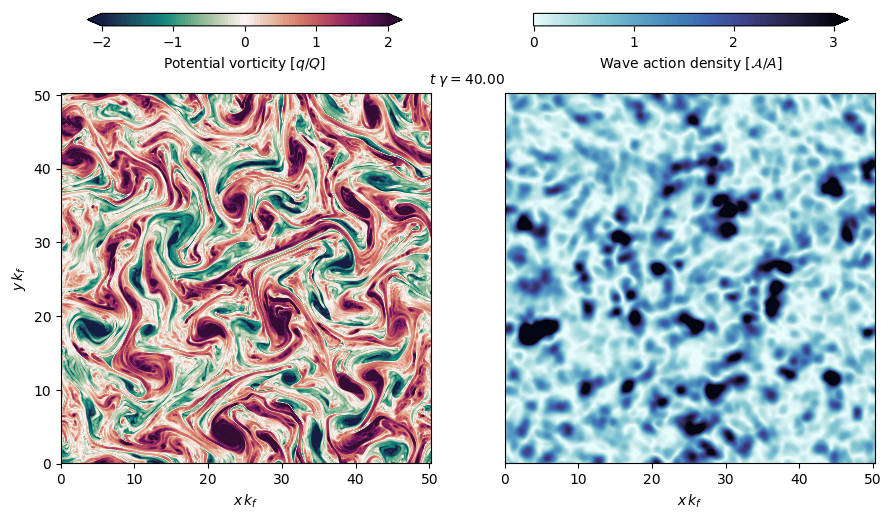
\includegraphics[width=.925\textwidth]{figs/snapshots_pv_qg-niw_reference.png}
\caption{Snapshot of potential vorticity and wave action density for the solution
         with parameters in  table \ref{parameters_reference}. The scale of potential vorticity
         is $Q = \sigma_q/\mu^{1/2} $ and the scale of wave action density is
         $A = \sigma_w^2/f_0 \gamma$.}
        \label{snapshots_pv_qg-niw_reference}
\end{figure}

Figure \ref{snapshots_pv_qg-niw_reference} shows snapshots of potential vorticity and wave
action density for a solution with $\sigma_w^2 = 2\sigma_q^2$ and $\gamma = 4\mu$; table
\ref{parameters_reference} describes in detail the parameters of
this reference solution. The equilibrated potential vorticity in figure
\ref{snapshots_pv_qg-niw_reference}a  resembles the vorticity field
of waveless two-dimensional turbulence with its ubiquitous eddies, filaments,
and coherent structures. A main difference is that the the potential vorticity
of this wave-modified turbulence is more fine-grained (see spectrum?).

The snapshot of wave action density depicts the incoherent nature of the equilibrated
wave field, which is being scrambled by the turbulent balanced field
(figure \ref{snapshots_pv_qg-niw_reference}b). The wave field develops scales smaller
than the balanced eddies due to straining by the flow and wave interference.
This snapshot resembles the wave field in decaying wave-modified
two-dimensional turbulence (RWY).

Figure \eqref{energies_reference} shows time series of balanced kinetic energy
and wave action and wave potential energy. The system equilibrates after $\sim\!1
\, \mu^{-1} = 4 \gamma^{-1}$. Wave action $\A$ displays large fluctuations ($50\%$ of
 the time-average equilibrated value). Balanced kinetic energy $\K$
and wave potential energy $\P$, on the other hand, show much smaller fluctuations
($10\%$ of the equilibrated levels). Interestingly, $\K$ and $\P$ fluctuate
largely out of phase.

The wave kinetic energy equilibrate at 60\% of theoretical prediction for waveless
turbulence forced by white-noise: $\Ewn = \sigma_q^2/\mu$. And the wave potential
energy equilibrates at about $10\%$ of the wave kinetic energy level, which suggests
that stimulated generation plays a crucial role in the equilibration of forced
barotropic turbulence.  Indeed, figure \ref{energy_budgets_reference}a shows that
stimulated generation, $-(\Gamma_r+\Gamma_a)$ in \eqref{Ke}, contributes about half
of the sink of wave kinetic energy---bottom drag,
$-2\mu \K$ in  \eqref{Ke}, accounts for the other half. Wave streaming, $\Xi$ in
\eqref{Ke}, is small but significant; $\Xi$ contributes about 5\% source of $\K$.
See table X1 for details of the budget.

The wave potential energy budget (figure \ref{energy_budgets_reference}b) confirms that
linear dissipation $-2\gamma \P$ damps most of $\P$ created via stimulated generation;
the residual is smaller than $1\%$ (table X2). Similarly, linear dissipation
$-2\gamma \A$ removes virtually all the wave action
$\A$ input by the white-noise forcing. While the forcing input is nearly constant,
wave action and the linear dissipation are highly interment. Thus, vertical viscosity damps the waves
and the details of horizontal small-scale dissipation are irrelevant.

The balanced kinetic energy spectrum has a submesoscale spectrum much smaller the
one of waveless turbulence. Stimulated generation also appears to slow down the
inverse cascade of balanced kinetic energy: there's more energy at large-scales
in the spectrum of waveless turbulence. The wave action has a nearly flat spectrum
between the forcing scale $k_f$ and the dissipative scale $k_d$.

\begin{figure}
\centering
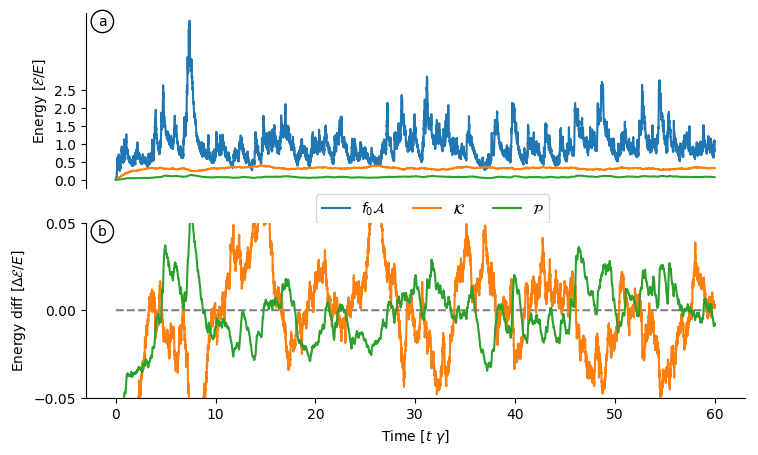
\includegraphics[width=.825\textwidth]{figs/energies_reference.png}
\caption{(a) Balanced kinetic energy ($\K$) and wave potential energy ($\P$) and wave
         kinetic energy ($f_0 \A$)  for the solution with parameters in table
         \ref{parameters_reference}. The energy difference, $\Delta \K$ and $\Delta \P$,
         about a time average after equilibration ($t\,\gamma \ge 5$).}
        \label{energies_reference}
\end{figure}

\begin{figure}
\centering
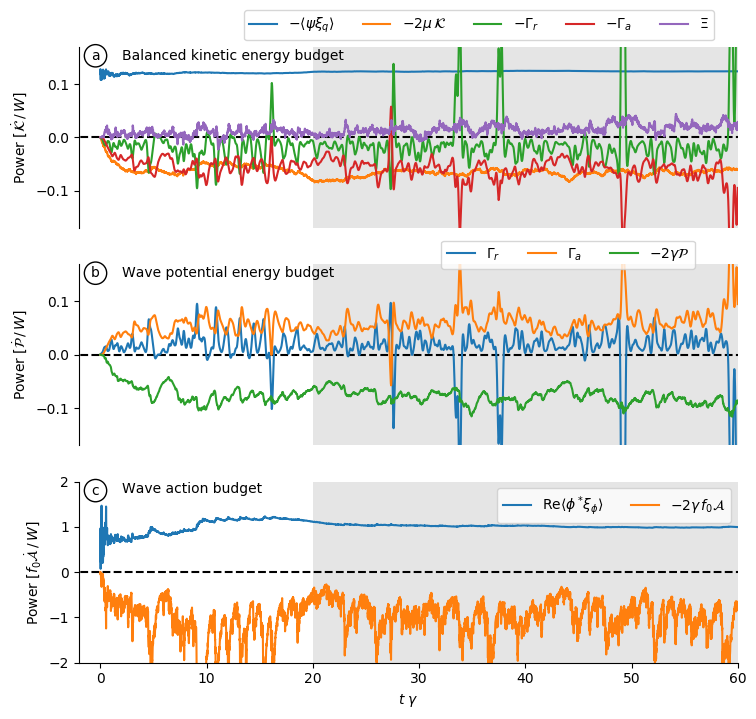
\includegraphics[width=.825\textwidth]{figs/K_and_P_and_A_budget_reference.png}
\caption{The budget of (a) balanced kinetic energy ($\K$), wave potential energy ($\P$),
        and (c) wave
         kinetic energy ($f_0 \A$)  for the solution with parameters in table
         \ref{parameters_reference}. The power is scaled by the work due to the
         wave forcing $W=\sigma_w^2/2$.}
        \label{energy_budgets_reference}
\end{figure}


\end{document}
